\documentclass{article}

\usepackage[utf8]{inputenc}
\usepackage{listings}
\usepackage{microtype}
\usepackage[english,dutch]{babel}
\usepackage[a4paper]{geometry}
\usepackage{graphicx}

\frenchspacing
\parindent=0pt
\setlength{\textheight}{25.7cm}
\setlength{\textwidth}{16cm}
\topmargin 260mm \advance \topmargin -\textheight
\divide \topmargin by 2 \advance \topmargin -1in
\headheight 0pt \headsep 0pt \leftmargin 210mm \advance
\leftmargin -\textwidth
\divide \leftmargin by 2 \advance \leftmargin -1in
\oddsidemargin \leftmargin \evensidemargin \leftmargin


\lstset{language=Python, showstringspaces=false, basicstyle=\small,
  numbers=left, numberstyle=\tiny, numberfirstline=false, breaklines=true,
  stepnumber=1, tabsize=4, 
  commentstyle=\ttfamily, identifierstyle=\ttfamily,
  stringstyle=\itshape, }
\title{Billiards}
\author{Luuk - s2260018\\levi van Es - s2115409 }
\date{November 2018}

\begin{document}

\maketitle

\section{Introduction}
    Deze opdracht was nogal drastisch anders dan de voorgaande. Het werd ons bij de eerste analyse van de opdracht al meteen duidelijk dat de opdracht de focus probeerde te leggen op het implementeren en gebruiken van classes. Gelukkig hebben we beide al enige ervaring met class achtige elementen uit andere object georienteerde programmeertalen en was het concept voor ons niet vreemd. 
    
\section{Code}
\subsection{Interface}
De gebruikers interface waar de gebruiker als eerst mee geconfronteerd word moest makkelijk en duidelijk in gebruik zijn met zo min mogelijk interactie en zo veel mogelijk resultaat. De wijze waarop dit moest gebeuren was zeer duidelijk gemaakt in de opdracht en was daarom ook niet heel moeilijk om te implementeren. Bij deze interface kwamen veel elementen terug uit vorige opdrachten en konden dus simpel met elkaar geintegreerd worden en aangepast worden aan dit programma. \newline Tot de huidige versie is er maar een enkel probleem dat zich optreed wanneer de handmatige invoer word verwerkt. Dit probleem komt naar voren wanneer er waardes voor de x worden ingevoerd die niet op het tafelvlak bevinden. Hier zijn overduidelijke oplossingen voor maar voor functionele doeleidnen hebben wij op het moment dit probleem opgelost door gebruik te maken van de modulus over de inputwaarde. Hierdoor krijgen we altijd een waarde binnen de dementies van de tafel. \newline De automatische invoer is compleet gebouwd op de numpy functie np.loadtxt. Deze functie is perfect voor het omzetten van text in een array. Wanneer dit is gebeurd is het maar een kwestie van de juiste waarde uit de array op de goede plek in de 2 dementionale positie array te zetten en dat was het.
\subsection{Plotting}
\subsubsection{(v,t)plot}
Het v,t plot is misschien nog wel het meest invoudige gedeelte van dit project. Omdat de snelheidsvectors opgeslagen staan in een chronologische lijst is het heel makkelijk om met pyplot gewoon de 1-dementionale snelheid van elke vector te plotten. Dit was ook de laatste implementatie die wij hebben gemaakt aan het programma. 
\subsubsection{Billiardplot}

\subsubsection{ASCII-Plot}
Het ASCII-Plot was bij de eerste gedachte een fluitje van een cent. Maar bij het verder lezen moest ook dit stuk van de code volgens een bepaalde manier gecodeerd worden. Hierbij moest een onbekende numpy functie gevonden worden die gebruikt moest worden om de 2 dementionale array/lijst om te zetten naar een genormaliseerde versie hiervan. Het vinden van deze functie bleek nog een groter opgeve dan gedacht. Vandaar dat het even duurde voor deze was geimplementeerd. 
De algemene opstelling van de ascii-plot code is als volgt. De code genereerd een 1 dementionale lijst met een | gevolgd door 70 spaties en vervolgens ee | en  een "\n". Door de x en de y coordinaten door een formule te halen komen we erachter welk element van de lijst we moeten vervangen door een x of een o. Dit resulteerd in een grafiek als volgt. 


\begin{figure}
\begin{verbatim}
+----------------------------------------------------------------------+ 
|                                      o                               | 
|                                      o                               | 
|                                      o                               | 
|                                      o                               | 
|                                      o                               | 
|                                      o                               | 
|                                      o                               | 
|                                      o                               | 
|                                      o                               | 
|                                      o                               | 
|                                                                      | 
|                                                                      | 
|                                                                      | 
|                                                                      | 
|                                                                      | 
|                                                                      | 
|                                                                      | 
|                                                                      | 
+----------------------------------------------------------------------+ 
\end{verbatim}
\caption{Ascii-plot van voorbeelddata}
\label{fig:ascii-box}
\end{figure}
\begin{figure}
  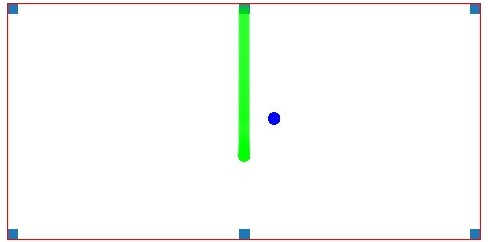
\includegraphics[width=\linewidth]{sampleplot.jpg}
  \caption{Reference correct plot}
  \label{fig:exampleplot}
\end{figure}
\newpage

Zoals we kunnen zien komt de grafiek 1 op 1 overeen met de verwachtte grafiek. Dit was voor ons een indicatie dat wij op het goede pad zaten en misschien nog maar een paar kleine aanpassingen moesten maken. De problemen waar wij hier tegenaanliepen waren voornamelijk de limitaties die ons werden opgelegd door de opdracht zelf. Verder duurde het even voordat het plan van aanpak voor dit plot op was gesteld. De realisatie van dit plan van aanpak bleek ook niet 1 op 1 vertaalbaar te zijn. Als gevolg moest er een hoop aanpassingen gedaan worden om tot deze uitkomst te komen.  

\section{Tijdsverdeling}

\begin{tabular}{ l | p{6cm} p{6cm} }
   & Luuk & Levi \\
  \hline
  Week 1 & Begonnen aan de implementatie van de classes en de muurdetectie per bal &  Begonnen aan de implementatie van de classes en de muurdetectie per bal \\
  Week 2 & Een begin maken aan Decodeerfunctie en ideen opdoen voor palindroomuitwerking & Begin maken aan user interface en zijn subsystemen(automatisch, handmatig) \\
  Week 3 & -Ideeen opdoen voor verdere decodeeroptimalisatie en aanpassingen maken aan de decodeerfunctie om de code zo efficient en klein mogelijk te maken.\linebreak -Integratie van palindroomfunctie in de decodeerfunctie & -Integratie invoersubsystemen in de userinterface en uitvoer formatting naar het juiste formaat voor de rest van de code  \\
  Week 4  & Debuggen van speciale gevallen bij het en- en decoderen. Implementeren van het compressieratio & Ontwikkelen en implementeren van ASCII-grafiek.   \\
 
 
 
  
\end{tabular}

\section{Code}

 \begin{lstlisting}[frame=single, language=python]
 
 
 
 \end{lstlisting}

\end{document}
